\documentclass[12pt, a4paper]{article}
\usepackage[utf8]{inputenc}
\usepackage{amsmath}
\usepackage{amsthm}
\usepackage{graphicx}
\usepackage{parskip}
\usepackage{hyperref}
\usepackage{fancyhdr}
\usepackage{lastpage}
\usepackage{color}
\usepackage{caption}
\usepackage{float}
\usepackage[vlined,ruled]{algorithm2e}
\usepackage[acronym]{glossaries}
\usepackage[nottoc]{tocbibind}
\usepackage{tikz}
\graphicspath{{./images/}}

\title{%
      Homework 4 \\
      X-Means Analysis as Efficient Estimation \\
      in the Number of Cluster
}
\author{%
  Juan Pablo Royo Sales\\
  \small{Universitat Politècnica de Catalunya}
}
\date\today

\pagestyle{fancy}
\fancyhf{}
\fancyhead[C]{}
\fancyhead[R]{Juan Pablo Royo Sales - UPC MIRI}
\fancyhead[L]{ADM - X-Means}
\fancyfoot[L,C]{}
\fancyfoot[R]{Page \thepage{} of \pageref{LastPage}}
\setlength{\headheight}{15pt}
\renewcommand{\headrulewidth}{0.4pt}
\renewcommand{\footrulewidth}{0.4pt}

\newacronym{kdt}{K-d Tree}{K-Dimensional Binary Search Tree}
\newacronym{xmean}{X-Means}{X-Means}
\newacronym{kmean}{K-Means}{K-Means}
\newacronym{voronoi}{Voronoi}{Voronoi Boundaries}
\newacronym{bic}{BIC}{Bayesian Information Criterion}

\begin{document}

\maketitle

\medskip

\section{Introduction}
In this article I am going to analyse in deep the paper publish in 2002 by \textbf{Pelleg and Moore} about \acrfull{xmean} \cite{xmean} as an efficient algorithm to estimate the number of cluster in the \acrfull{kmean} Algorithm.

Basically the authors claimed in the paper that \acrshort{kmean} suffer for 3 main problems that they try to address with \acrshort{xmean}: one of the problem is that \acrshort{kmean} is slow and it scales bad with regards to the time it takes an iteration to complete. Secondly the parameter \textbf{K} which is the number of cluster is need to be provided beforehand by the user, and finally static number of cluster finds worse local optima rather than dynamic K.

Regarding the performance in relation to execution time, this has been achieved using a \acrfull{kdt} to store the dataset, taking advantage of two geometric techniques: \acrfull{voronoi} \cite{geometric_2} and \textit{blacklisting} to maintain a list of those centroids that needs to be considered for a given region \cite{geometric}. This last technique is used as a core of \acrshort{xmean} in order to estimate \textbf{K}.

Basically the algorithm split the centroids in order to best fit the data. This splitting is dong computing \acrfull{bic}. In the analysis is shown that doing this does not cost more than 1 \acrshort{kmean} iteration. Also caching techniques are applied to not recompute data.


\section{Estimation of K}
As we have described in the introduction with this new approach the user does not specified the number of \textbf{K} beforehand, but it is required that the user provides a possible range in where this \textbf{K} falls.

\subsection{Model Searching}
The algorithm starts with the lower bound \textbf{K} provided in the ranged and continues adding centroids meanwhile are needed until it reach the upper bound. The one with the best \textit{score} at the end is the one selected.

\begin{algorithm}[H]
  \SetKwInOut{Input}{Input}
  \SetKwInOut{Output}{Output}
\Input{Given $R = (l,b)$ Range of K}
  \Output{$C$ Centroid set with the best score}
  $K \longleftarrow 1$\;
  $C \longleftarrow \emptyset$\;
  \While{$K <= b$}
  {\emph{Improve Params} \tcp*[f]{Running convergence K-Mean}\;
    \emph{Improve Structure} \tcp*[f]{See details bellow~\ref{sub:sub:imp:struct}}\;
    \If{Centroid $c$ with best score was found~\ref{sub:bic}}
    {$C \longleftarrow C \cup \{c\}$
    }
    $K \longleftarrow K + 1$
  }
  return $c$;
  \caption{\acrshort{xmean} Algorithm}
\end{algorithm}

\subsubsection{Improve Structure}\label{sub:sub:imp:struct}
This step of the algorithm basically finds out where the new centroids should appear. There are 2 possible strategies on doing this, one is to pick a centroid and find a nearest one, but this would take at least $O(K_{\text{max}})$ to be perform.

Another strategy to do this is to \textit{try half of the centroids}, which choose half of the centroid according to some heuristic on how promising they are to be split. This requires only $O(\log{K_{\text{max}}})$. The problem with this strategy is how to choose the heuristic.

In both strategies, after doing this we run \acrlong{kmean} and if it scores better we keep new centroids or we discard otherwise.

In \acrlong{xmean} algorithm we used both strategies in the following way:

\begin{algorithm}[H]
  \SetKwInOut{Input}{Input}
  \SetKwInOut{Output}{Output}
  \Input{Given set of Centroids $C$}
  \Output{$C'$ New Centroid set with best fit}
  $C' \longleftarrow \emptyset$\;
  \ForEach{$c \in C$}
  {$(a,b) \longleftarrow \text{Split } c \text{ in two Centroids}$\;
    \emph{Run local K-mean with $K = 2$ and $(a,b)$ as new Centroid}\;
    \If{$(a,b)$ are modeling real Centroid structure for this region}
    {$C' \longleftarrow C \cup \{a,b\}$
    }
  }
  return $C'$;
  \caption{\acrshort{xmean} Improve Structure Algorithm}
\end{algorithm}



\begin{itemize}
  \item Split each centroid into 2 children with a distance proportional to the size of the region~\ref{fig:centroid_split} in a random chosen vector
  \item Run local \acrlong{kmean} in each parent region with $K = 2$.
  \item Model selection test is run on all pair of children. Are this children modeling a real structure?
  \item If the answer is yes, keep those centroids, otherwise discard.
\end{itemize}

\begin{minipage}[f]{\linewidth}
  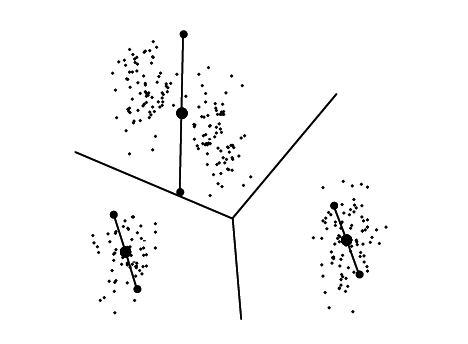
\includegraphics[width=\textwidth]{xmeans_1}
  \captionsetup{type=figure}
  \captionof{figure}{Example of Centroid splitting}
  \label{fig:centroid_split}
\end{minipage}

\subsection{BIC Scoring}\label{sub:bic}
Given a data $D$ and a set of alternative family models $M_j$, in order to score each model we are going to use posterior probabilities $P[M_j|D]$.

To do posterior approximation it is used the formula from \cite{bic}:

\begin{equation}
BIC(M_j) = \widehat{l}_j(D) - \frac{p_j}{2} \times \log{R}
\end{equation}

\begin{itemize}
  \item $\widehat{l}_j$ is the $\log$-likelihood of the data according to the $j$-th model.
 \item $p_j$ Number of parameters in $M_j$
\end{itemize}

The $\log$-likelihood is:

\begin{subequations}
  \begin{align}
  l(D) &= \log{\prod_i P(x_i)}\\
  &= \sum_i \left( \log{\frac{1}{\sqrt{2\pi}\sigma^M}} - \frac{1}{2\sigma^2} \mid\mid x_i - \mu_{(i)} \mid\mid^2 + \log{\frac{R_{(i)}}{R}} \right)\label{eq:1}
  \end{align}
\end{subequations}

The maximum estimate likelihood is:

\begin{equation}
  \widehat{\sigma}^2 = \frac{1}{R - K} \sum_i \left( x_i - \mu_{(i)} \right)^2\label{eq:2}
\end{equation}

Plug-in~\ref{eq:1} and~\ref{eq:2} we have:

\begin{equation}
  \widehat{I}(D) = -\frac{R_n}{2} \log{2\pi} - \frac{R_n \times M}{2} \log{\widehat{\sigma}^2} - \frac{R_n - K}{2} + R_n\log{R_n} - R_n \log{R}
\end{equation}

To extend this formula to all centroids, since we know that the $\log$-likelihood of the points that belongs to all centroids is the sum of the $\log$-likelihood of individual centroids, we can replace $R$ which the total number of points that belongs to the Centroid $c$ under consideration.

\subsection{Boosting Performance}
In this section we are going to describe a couple of techniques used in order to speed up the algorithm in all its phases.

\begin{itemize}
  \item \textbf{Speeding K-Means:} To speed up \acrlong{kmean} algorithm we are going to store statistics data in order to save computations after. This is done using a \acrlong{kdt} structure where each $kd$-node represents a subset of the data set. Basically this is done maintaining counters for each centroid with the number of points that belongs to it as well as their vector sum. Using a \acrshort{kdt} allows us to update this numbers navigating the structure only once.

  \item \textbf{Speeding Improve Structure:} In this case the same structure (\acrshort{kdt}) is used in order to collect data regarding the centroid location on each iteration, plus a list to do the division on the children centroids recursing from the bigger list with all centroids to the bottom with 2.

  \item \textbf{Additional Speed up:} An additional improve is the comparison of centroid location. In order to achieve constant access for comparing centroid a data structure with write-once feature is used in order to not permit alterations of the centroid coordinates. Basically a \textbf{HashMap}-like structure is used and each centroid is assigned with a new identifier each time it is discovered. In this way if a centroid change position, we insert a new centroid with a new identifier and its own coordinates.
\end{itemize}

\section{Experimental Results}
In the paper \cite{xmean} we can see the analysis and results of experiments that the authors has conducted that we can sum up in the following list:

\begin{itemize}
  \item Regarding speed it has shown that \acrshort{xmean} runs twice as fast for larger problems regarding \acrshort{kmean}
  \item The quality in terms of \acrshort{bic} and distortion was superior for \acrshort{xmean}
  \item The average cluster size is smaller for \acrshort{xmean} rather than \acrshort{kmean}
  \item Running time is not only fast but also it scales better when the number of points increases
\end{itemize}

\section{Conclusion}
\acrfull{xmean} has been presented in the paper as an improvement of \acrshort{kmean} algorithm tackling down the issues that \acrshort{kmean} presents.

It has shown that using techniques like \acrshort{bic}, data structures for locating geometric data \acrshort{kdt} and also implementing caching can improve \acrshort{kmean} in superior way in terms of performance and scalability.

Another important point is the ability of the algorithm to predict $K$ value at the same time that the clustering process is taking place.

In that sense I think it is a good algorithm that can be taken into consideration as an implementation or specialization of \acrshort{kmean}.

\bibliographystyle{alpha}
\bibliography{Homework4_jproyo}

\end{document}

